\documentclass[a4paper, 16pt]{article}
\usepackage[UTF8]{ctex}
\usepackage{geometry}
\usepackage{graphicx}
\usepackage{setspace}
\usepackage{float}
\usepackage{listings}
\usepackage{xcolor}
\usepackage{multirow}
\lstset{
    numbers=left, 
    numberstyle= \tiny, 
    keywordstyle= \color{ blue!70},
    commentstyle= \color{red!50!green!50!blue!50}, 
    frame=shadowbox, % 阴影效果
    rulesepcolor= \color{ red!20!green!20!blue!20} ,
    escapeinside=``, % 英文分号中可写入中文
    xleftmargin=5em,xrightmargin=5em, aboveskip=2em,
    framexleftmargin=2em
} 
\geometry{left = 1.0 cm, right = 1.0cm, top = 2.0cm, bottom = 2.0cm	}
\title{编译原理第八章(二)}
\author{李鹏辉}

\begin{document}
\maketitle

1.(8.4.1)图8-10是一个简单的矩阵乘法程序。

1)假设矩阵的元素是需要8个字节的数值,而且矩阵按行存放。把程序翻译成为我们本节中使用的那种三地址语句。

2)为1)中得到的代码构造流图

3)找出在2)中得到的流图的循环


\lstset{language=C}
\begin{lstlisting}
for (i = 0; i < n; i ++)
	for(j = 0; j < n; j ++)
		c[i][j] = 0.0;
for (i = 0; i < n; i ++)
	for(j = 0; j < n; j ++)
		for(k = 0; k < n; k ++)
			c[i][j] = c[i][j] + a[i][k]*b[j][j];

\end{lstlisting}

生成三地址代码如下所示
\begin{table}[H]
\centering
\begin{tabular}{l l}
B1&1) i = 0\\
B2&2) if i $>=$ n goto 13) \\
B3&3) j =0 \\
B4&4) if j $>=$ n goto 11) \\
B5&5) t1 = n*i \\
&6) t2 = t1 + j\\
&7) t3 = t2*8\\
&8) c[t3] = 0.0\\
&9) j = j + 1\\
&10) goto 4)\\
B6& 11) i = i + 1\\
& 12) goto2) \\
& \\
B7&13) i = 0 \\
B8&14) if i $>=$ n goto 40) \\
B9&15) j = 90 \\
B10& 16) if j $>=$ n goto 38) \\
B11& 17) k = 0\\
B12& 18) if k $>=$ n goto 36)\\
B13&19) t4 = n*i\\
&20) t5 = t4 + j\\
&21) t6 = t5*8\\
&22) t7 = c[t6]\\
&23) t8 = n * i\\
&24) t9 = t8 + k\\
&25) t10 = t9*8 \\
&26) t11 = a[t10]\\
&27) t12 = n * k\\
&28) t13 = t12 + j\\
&29) t14 = t13 + j\\
&30) t15 = b[t14]\\
&31) t16 = t11 * t15\\
&32) t17 = t7 + t16\\
& 33) c[t6] = t17\\
&34) k = k + 1\\
&35) goto 18)\\

B14&36) j = j + 1\\
&37) goto 16)\\
B15&38) i = i + 1\\
& 39) goto 14)\\
\end{tabular}
\end{table}

流图如下

\begin{figure}[H]
\centering
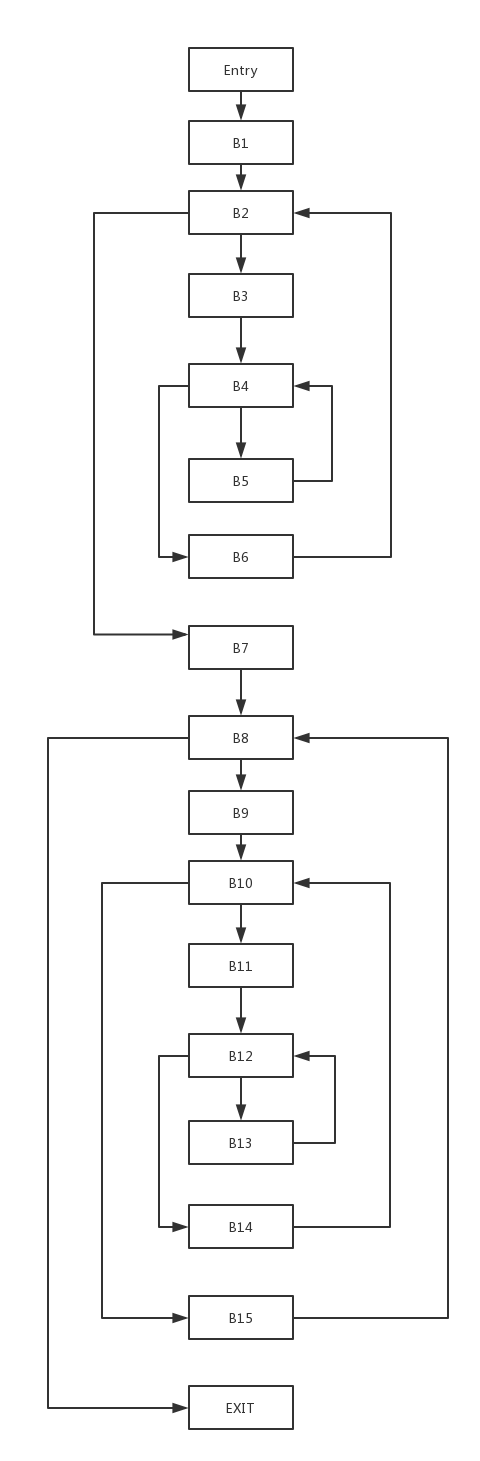
\includegraphics[scale=0.5]{chapter8_hw2_1}
\end{figure}
如上图所示,我们可以找到循环如下

$B2,B3,B4,B5,B6$

$B4,B5$

$B8,B9,B10,B11,B12,B13,B14,B15$

$B10,B11,B12,B13,B14$

$B14,B15$

2.(8.5.1)为下面的基本快构造DAG,并假设只有a在基本快出口活跃,简化下面三地址代码。
\lstset{language=C}
\begin{lstlisting}
d = b + c
e = a + b
b = b * c
a = e - d
\end{lstlisting}
\begin{figure}[H]
\centering
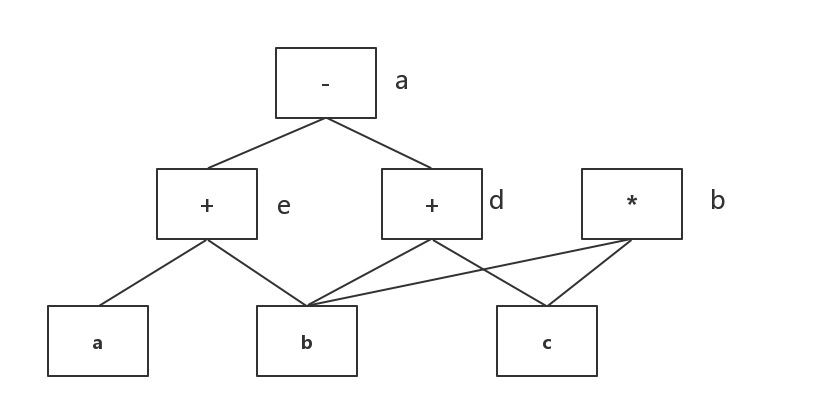
\includegraphics[scale=0.5]{chapter8_hw2_2}
\end{figure}
代码可以简化为

\lstset{language=C}
\begin{lstlisting}
d = b + c
e = a + b
a = e - d
\end{lstlisting}
\end{document}